\chapter{Исследовательский раздел}
В разделе представлены результаты проведенного эксперимента, в котором сравниваются временные характеристики работы реализованного программного обеспечения.
 
\section{Технические характеристики}
Технические характеристики устройства, на котором выполнялось тестирование:
\begin{itemize}
	\item операционная система: Ubuntu 21.10;
	\item память: 8 ГГц;
	\item процессор: Intel(R) Core(TM) i5-8265U CPU @ 1.60 ГГц   1.80 ГГц.
\end{itemize}

Во время тестирования устройство было подключено к блоку питания и не нагружено никакими приложениями, кроме встроенных приложений окружения и самим окружением.

\section{Апробация}
На рисунках \ref{png:result_landscape_1} - \ref{png:result_landscape_5} представлены результаты синтеза изображения с различными параметрами ландшафта и освещенности сцены.
\begin{figure}[H]
	\centering{
		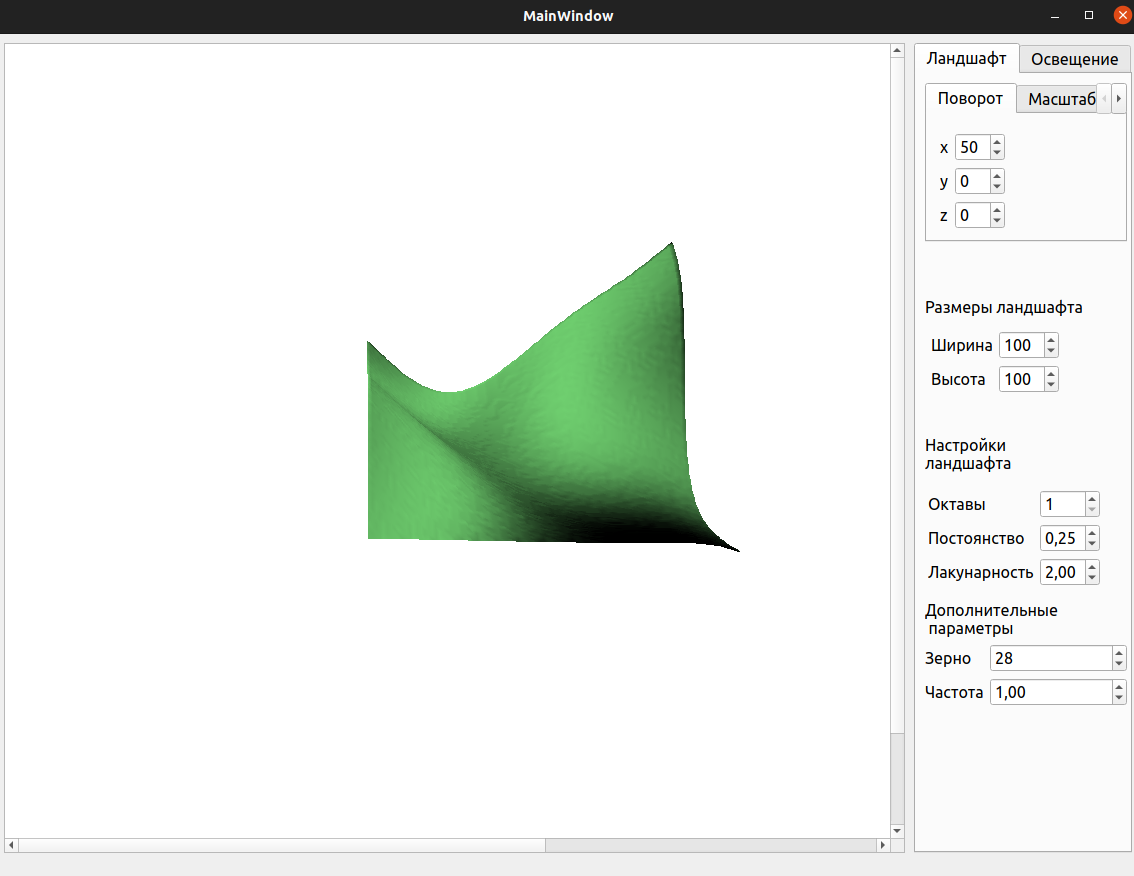
\includegraphics[scale=0.35]{../../../../../../../msys64/home/Лев/bmstu_cg_course_project/rpz/images/landscape_4}
		\caption{Визуализация сцены в обычном режиме}
		\label{png:result_landscape_1}
	}
\end{figure}

\begin{figure}[H]
	\centering{
		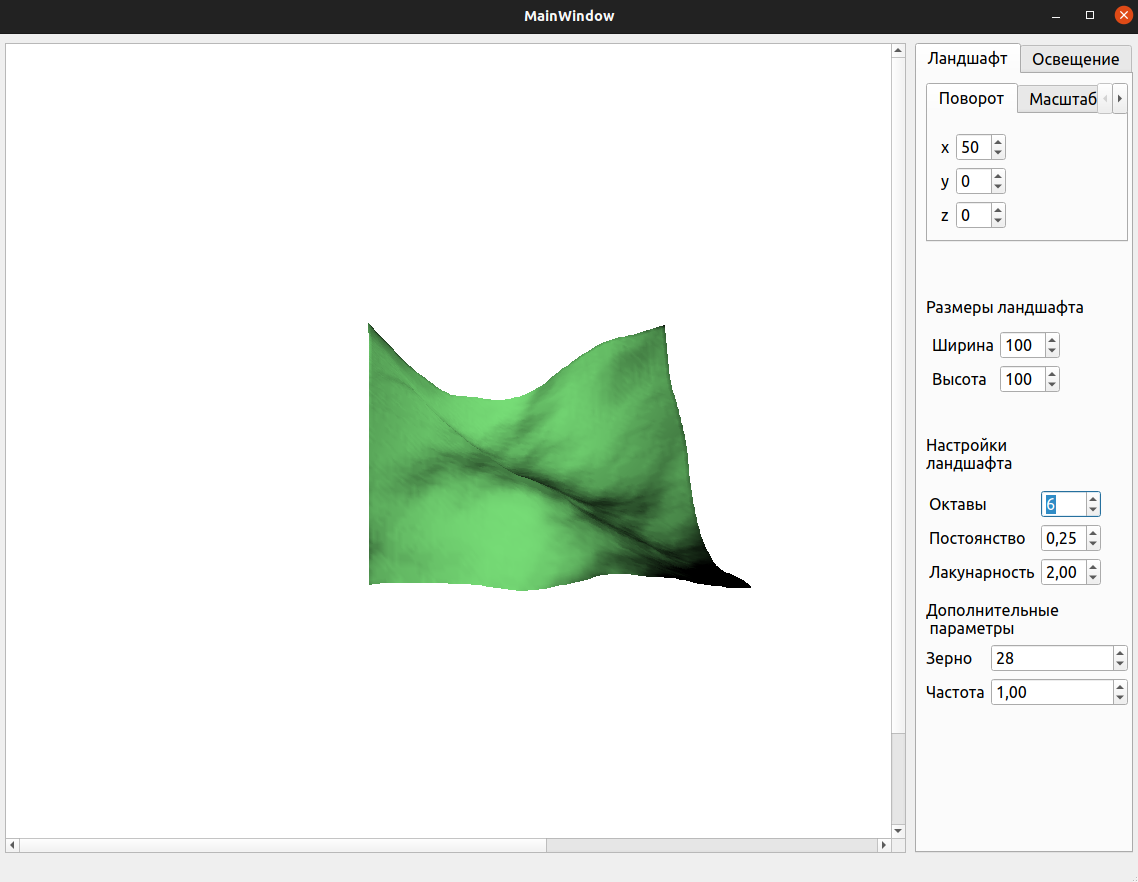
\includegraphics[scale=0.35]{../../../../../../../msys64/home/Лев/bmstu_cg_course_project/rpz/images/landscape_7}
		\caption{Применение нескольких октав к исходному ландшафту}
		\label{png:result_landscape_2}
	}
\end{figure}

\begin{figure}[H]
	\centering{
		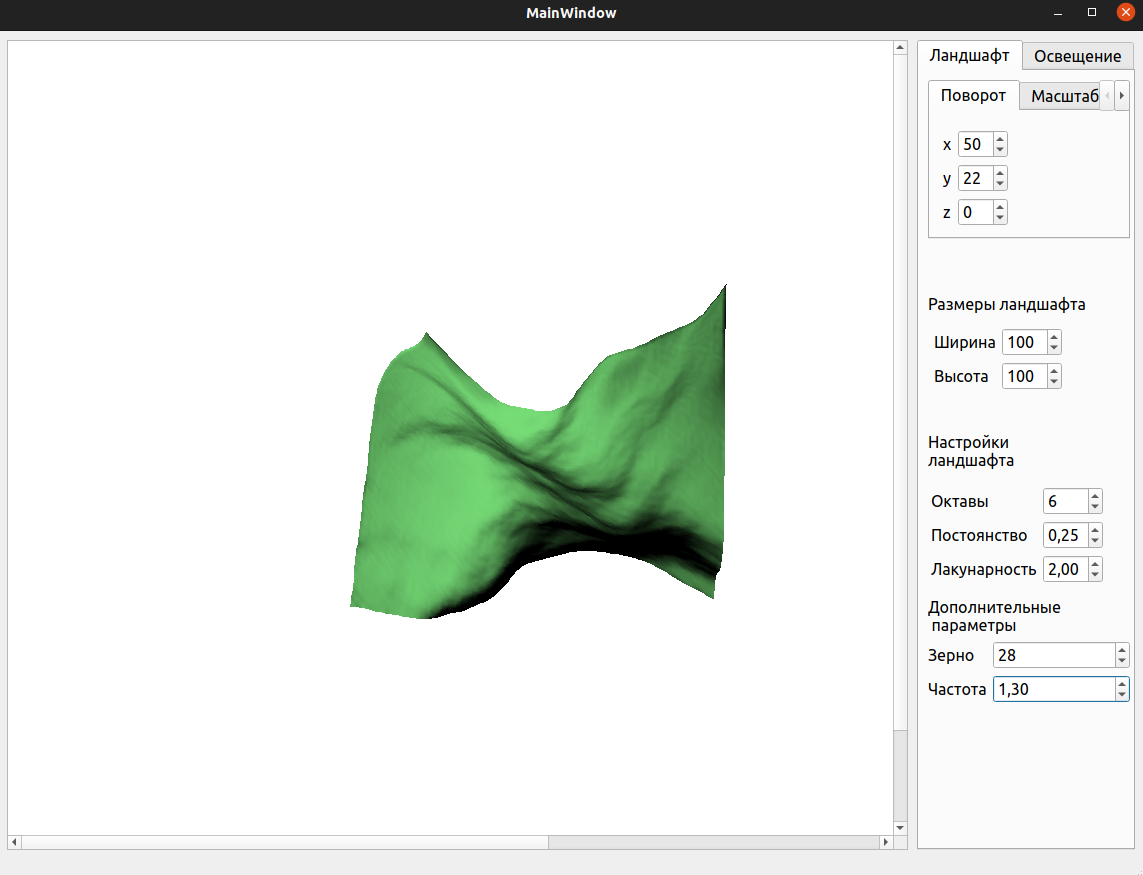
\includegraphics[scale=0.35]{../../../../../../../msys64/home/Лев/bmstu_cg_course_project/rpz/images/landscape_6}
		\caption{Изменение частоты исходного ландшафтаы}
		\label{png:result_landscape_3}
	}
\end{figure}

\begin{figure}[H]
	\centering{
		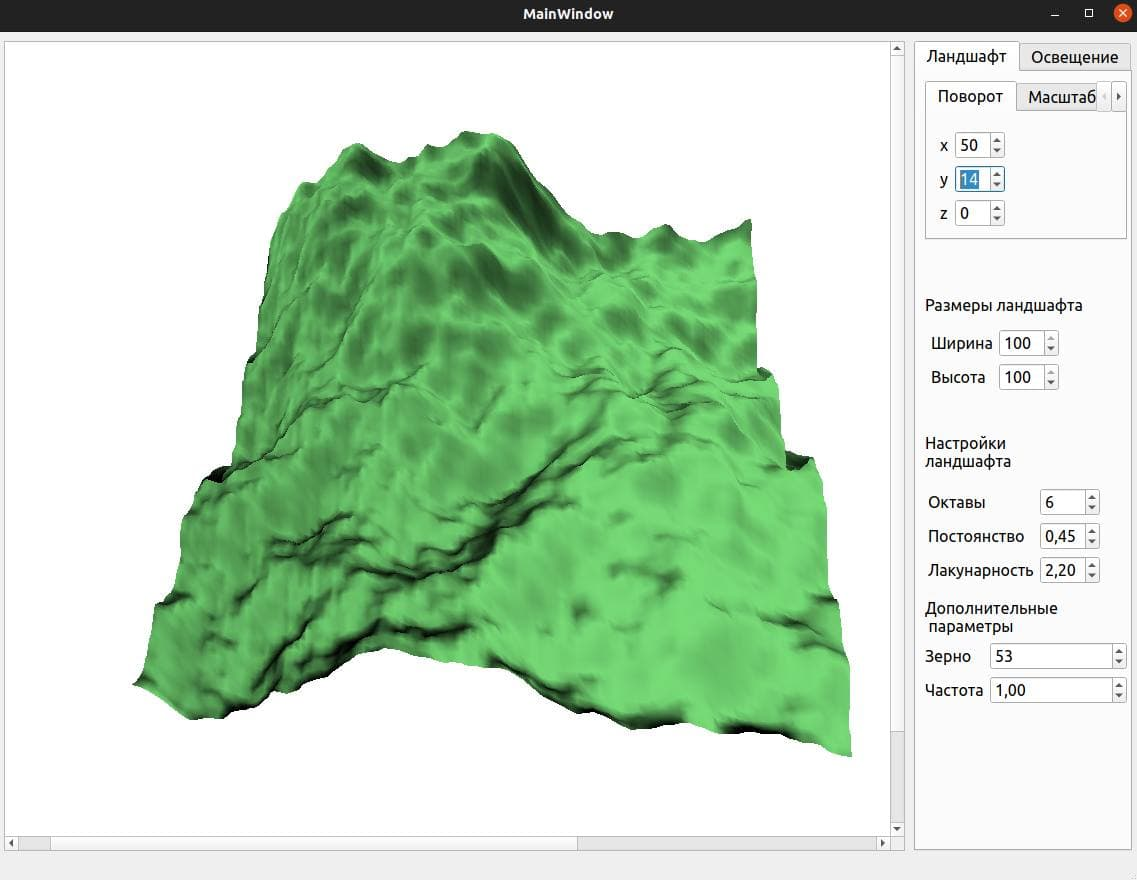
\includegraphics[scale=0.6]{../../../../../../../msys64/home/Лев/bmstu_cg_course_project/rpz/images/landscape_3}
		\caption{Изменение параметра "зерно"\ ландшафта}
		\label{png:result_landscape_4}
	}
\end{figure}

\begin{figure}[H]
	\centering{
		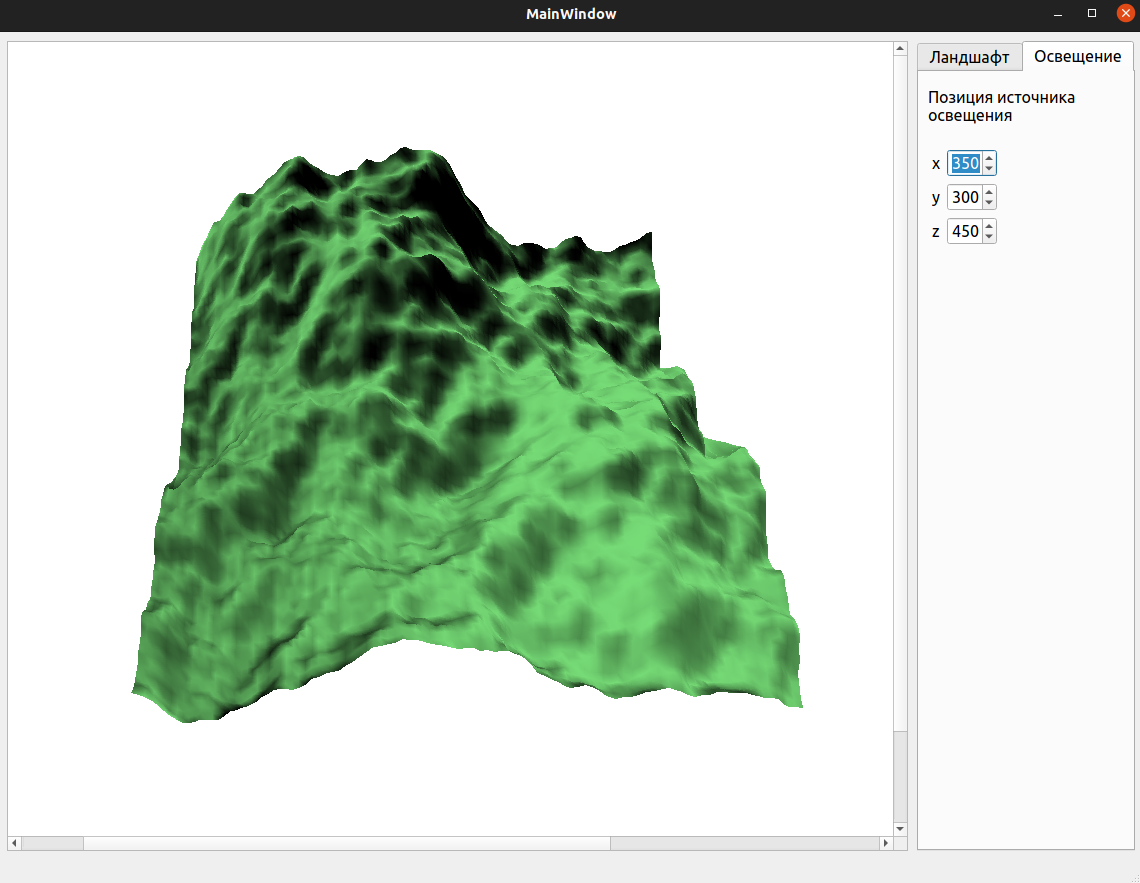
\includegraphics[scale=0.35]{../../../../../../../msys64/home/Лев/bmstu_cg_course_project/rpz/images/landscape_5}
		\caption{Изменение позиции источника освещения}
		\label{png:result_landscape_5}
	}
\end{figure}



\section{Постановка первого эксперимента}
Целью эксперимента является определение зависимости времени отрисовки ландшафта от количества полигонов сетки, разбитых на треугольники. Эксперимент проводился на ландшафте, имеющем размер $10\times10$, $25\times25$, $50\times50$, $100\times100$, $150\times150$, $250\times250$, $350\times350$, $500\times500$.

Для снижения погрешности измерений один и тот же эксперимент будет проведен в количестве N=10, после что будет вычислять среднеарифметическое значение измеряемой величины.


\section{Результат первого эксперимента}
В таблице \ref{table:draw_landscape} приведены экспериментально полученные значения временных характеристик отрисовки ландшафта.

\begin{table}[ht!]
	\centering
	\captionsetup{singlelinecheck = false, justification=raggedright}
	\caption{Таблица времени визуализации ландшафта в зависимости от его линейного размера (в секундах).}
	\label{table:draw_landscape}
	\begin{tabular}{|c|c|}
		\hline
		Размер & Время \\ \hline
		10 & 0.336509 \\ \hline
		25 & 0.32979 \\ \hline
		50 & 0.342097 \\ \hline
		100 & 0.387329 \\ \hline
		150 & 0.468589 \\ \hline
		250 & 0.721446 \\ \hline
		350 & 1.06574 \\\hline
		500 & 2.02038 \\\hline
		700 & 19.6004 \\\hline
	\end{tabular}
\end{table} 

На рисунке \ref{fg:ref1} приведена зависимость времени отрисовки изображения от линейного размера ландшафта (в секундах).

\begin{figure}[H]
	\centering
	\captionsetup{justification=centering}
	\begin{tikzpicture}
		\begin{axis}
			[grid = major,
			xlabel = Размер ландшафта,
			ylabel = {Время, c},
			ymin = 0,
			width = 0.95\textwidth,
			height=0.3\textheight,
			legend style={at={(0.5,-0.2)},anchor=north},
			xmajorgrids=true]
			\addplot table{data/visualization_time.txt};
			\legend{
				Визуализация ландшафта
			};
		\end{axis}
	\end{tikzpicture}
	\caption{Зависимость времени отрисовки ландшафта от его линейного размера.} 
	\label{fg:ref1}
\end{figure} 


\section{Постановка второго эксперимента} 
Целью эксперимента является определение скорости формирования карты высот на основе шума Перлина в зависимости от числа октав для размера ландшафта $100\times100$. Диапазон значений октав берется от 1 до 8. Большее число октав не рассматривается, так как пользователю будет уже неразличим отрисованный на экране результат.

\section{Результат второго эксперимента}
В таблице \ref{table:draw_landscape} приведены экспериментально полученные значения временных характеристик формирования карты высот в зависимости от числа октав.

\begin{table}[ht!]
	\centering
	\captionsetup{singlelinecheck = false, justification=raggedright}
	\caption{Таблица времени формирования карты высот в зависимости от числа октав (в секундах).}
	\label{table:octaves}
	\begin{tabular}{|c|c|}
		\hline
		Октавы & Время \\ \hline
		1 & 0.000583146 \\ \hline
		2 & 0.00114126 \\ \hline
		3 & 0.00153122 \\ \hline
		4 & 0.0021004 \\ \hline
		5 & 0.00270201 \\ \hline
		6 & 0.00337686 \\ \hline
		7 & 0.0042514 \\\hline
		8 & 0.00541033 \\\hline
	\end{tabular}
\end{table} 

На рисунке \ref{fg:ref2} приведена зависимость времени формирования карты высот от числа октав (в секундах).

\begin{figure}[H]
	\centering
	\captionsetup{justification=centering}
	\begin{tikzpicture}
		\begin{axis}
			[grid = major,
			xlabel = Количество октав,
			ylabel = {Время, c},
			ymin = 0,
			width = 0.95\textwidth,
			height=0.3\textheight,
			legend style={at={(0.5,-0.2)},anchor=north},
			xmajorgrids=true]
			\addplot table{data/octaves_time.txt};
			\legend{
				Применение числа октав.
			};
		\end{axis}
	\end{tikzpicture}
	\caption{Зависимость времени работы алгоритма шума Перлина от числа октав.} 
	\label{fg:ref2}
\end{figure} 

\section{Вывод}
По результатам эксперимента можно сделать вывод о том, что формирование карты высот на основе шума Перлина с использованием нескольких октав требует разные временные затраты. Время выполнения программы для 4 октав медленнее времени выполнения для 1 октавы в 3,6 раз. Для количества октав 4 и 8 эта разница составляет 2,57 раз. При этом общее время визуализации ландшафта начинает увеличиваться с размера $500\times500$. Общее время для размера $700\times700$ отличается уже в 9,68 раз.